\documentclass[9pt,twocolumn]{paper-template}
% Use the lineno option to display guide line numbers if required.
\usepackage{float}
\usepackage{lipsum}
\usepackage{amsmath}
\usepackage{subcaption}
\usepackage{romannum}
\templatetype{twocolumn} % Choose template 
% {pnasresearcharticle} = Template for a two-column research article
% {pnasmathematics} %= Template for a one-column mathematics article
% {pnasinvited} %= Template for a PNAS invited submission

\title{Neuroscience Term Project}

% Use letters for affiliations, numbers to show equal authorship (if applicable) and to indicate the corresponding author
\author[a,b]{Ali Hassanzadeh Mahani}
\author[b,c]{Maedeh Karkhaneh Yousefi} 
\author[a]{Yaghoub Shahmari}

\affil[a]{Student, Physics Department, Sharif University of Technology}
\affil[b]{Affiliation Two}
\affil[c]{Affiliation Three}

% Please add here a significance statement to explain the relevance of your work
\significancestatement{You are encouraged to submit a 120-word maximum statement about the significance of your paper written at a level understandable to an undergraduate educated scientist outside their field of speciality. The primary goal of the Significance Statement is to explain the relevance of the work in broad context to a broad readership. The Significance Statement appears in the paper itself and is required for all research papers in some journals.}

% Please include corresponding author, author contribution and author declaration information
\authorcontributions{Please provide details of author contributions here.}
\equalauthors{\textsuperscript{1}A.O.(Author One) and A.T. (Author Two) contributed equally to this work (remove if not applicable).}

% Keywords are not mandatory, but authors are strongly encouraged to provide them. If provided, please include two to five keywords, separated by the pipe symbol, e.g:
\keywords{Keyword 1 $|$ Keyword 2 $|$ Keyword 3 $|$ ...} 

\begin{abstract}
Please provide an abstract of no more than 250 words in a single paragraph. Abstracts should explain to the general reader the major contributions of the article. References in the abstract must be cited in full within the abstract itself and cited in the text.
\end{abstract}

\dates{This manuscript was compiled on \today}

\begin{document}

\maketitle
\thispagestyle{firststyle}
\ifthenelse{\boolean{shortarticle}}{\ifthenelse{\boolean{singlecolumn}}{\abscontentformatted}{\abscontent}}{}

% If your first paragraph (i.e. with the \dropcap) contains a list environment (quote, quotation, theorem, definition, enumerate, itemize...), the line after the list may have some extra indentation. If this is the case, add \parshape=0 to the end of the list environment.
\dropcap{I}n this paper we have used the electrophysiological dataset recorded in motor cortex of two macaque monkey(N) during an instructed delayed reach-to-grasp task to create numerous plots. Meanwhile the data is recorded with a 10$ \times $10 electrode array. The area under control includes: central sulcus, M1, Premotor Cortex Dorsal (PMD) and Premotor Cortex Ventral (PMV). 96 electrodes out of 100 have the data we need.
We'll be clarifying the type of the process, whether the neurons are sensitive to a particle event or not, studying the firing rate based on different events, and etc. \citep{dataset}
\section*{Behavioural Task}
\paragraph*{}
The task is done by Monkey (N) and recorded during the trials. TS$ \_ $ON set signals when the task begins. After 400 ms, the yellow LED turns on, a signal that the start of the trial (WS$ \_ $ON). CUE$ \_ $ON set is the representation of how the monkey should grasp the object; Whether it is a side grip (SG) and the two left LEDs turn on, or it's a precision grip (PG) and the two right LEDs turn on. After 300 ms CUE$ \_ $OFF happens and the LEDs turn off. During the following 1000 ms, if something out of order happens, the trial leads to an error; and if not, at GO$ \_ $ON set, signal to the monkey to move its hand and grip the object divides into two kinds: Low force (LF) and high force (HF). After some delay, depending on the monkey's own behaviour, SR$ \_ $ON signals the start of the monkey's hand's motion. If no error happens, it should hold on the object for 500 ms, and then it receives the reward (RW$ \_ $ON). At last, WS$ \_ $OFF signals the end of the trial. These events are saved as bit numbers in dataset. 

\section*{Materials and Methods}
\paragraph*{} 
We used the data associated with the neurons' spike trains and the events during the trials. In order to have the raster plot, each trial has been separated from other trials, and its starting time shifted to zero. This way the behaviour of neurons can be seen during each trial. PSTH figure is the density of spikes over time, and is plotted with the same data sorting procedure (Fig. 2). Because the events were not altogether ordered and collected over time, showing the events as vertical line in Fig. 1 would cause unnecessary confusion. So, instead, a histogram of events for all the trials is provided, implementing which events have happened at which time during the trial (Fig. 3). The histogram plot of the ISI of all the trials is shown in Fig. 4. Of course, the trials are gone through a filter to eliminate the outlier data. 
nd should not be used. 

\begin{SCfigure*}[\sidecaptionrelwidth][H]
\centering
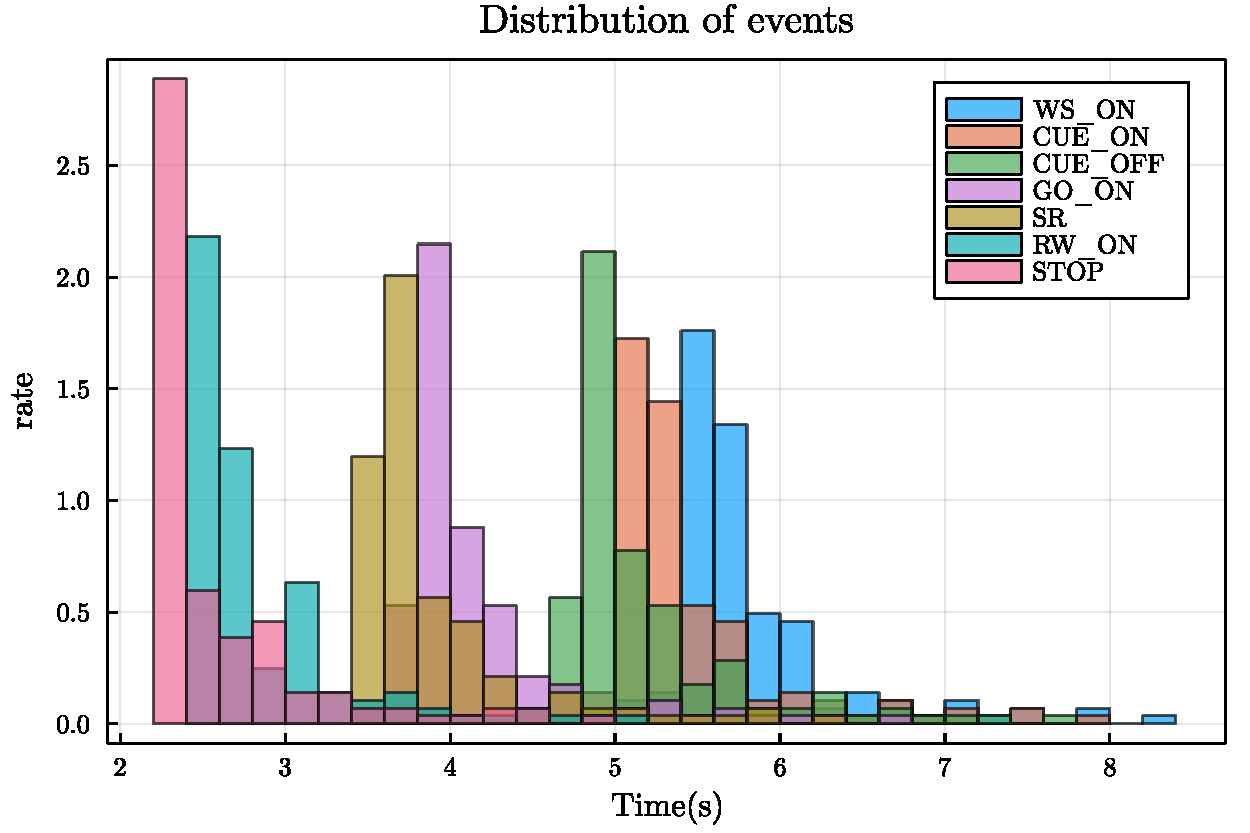
\includegraphics[width=12cm,height=11.4cm]{EvDist.pdf}
\caption{The density of events in all the trials over time.}\label{fig:side}
\end{SCfigure*}
\section*{Results}
Go over your analysis/experiments step by step and
describe what is shown in each figure then make a case
to go to the next analysis.\\


\section*{Discussion}
A stochastic process that generates a sequence of events, such as action
potentials, is called a \textbf{point process}. If the probability of an event occurring at any given time doesn't depend at all on the preceding events , so that the events themselves are statistically independent, we have a \textbf{Poisson process}. The \textbf{Homogeneous Poisson process}, which we are involved with here, causes the Poisson distribution: 
\begin{gather*}
P_{T}[n]=\frac{(r T)^{n}}{n !} \exp (-r T)\ \ \ \ (\Romannum{1})
\end{gather*}

The probability density of time intervals between adjacent spikes is called the interspike interval distribution (ISI), and it is a useful statistic for characterizing spiking patterns. From equation (\Romannum{1}), with n = 0, the probability of not firing a spike for period $ \tau $ is $ exp(-r\tau) $, so the probability of an interspike interval falling
between $ \tau $ and $ \Delta t + \tau $ is: 
\begin{gather*}
P\left[\tau \leq t_{i+1}-t_{i}<\tau+\Delta t\right]=r \Delta t \exp (-r \tau)\ \ \ \ \Romannum{2}
\end{gather*}
(dummy text)\lipsum[1]


\begin{SCfigure*}[\sidecaptionrelwidth][t]
\centering
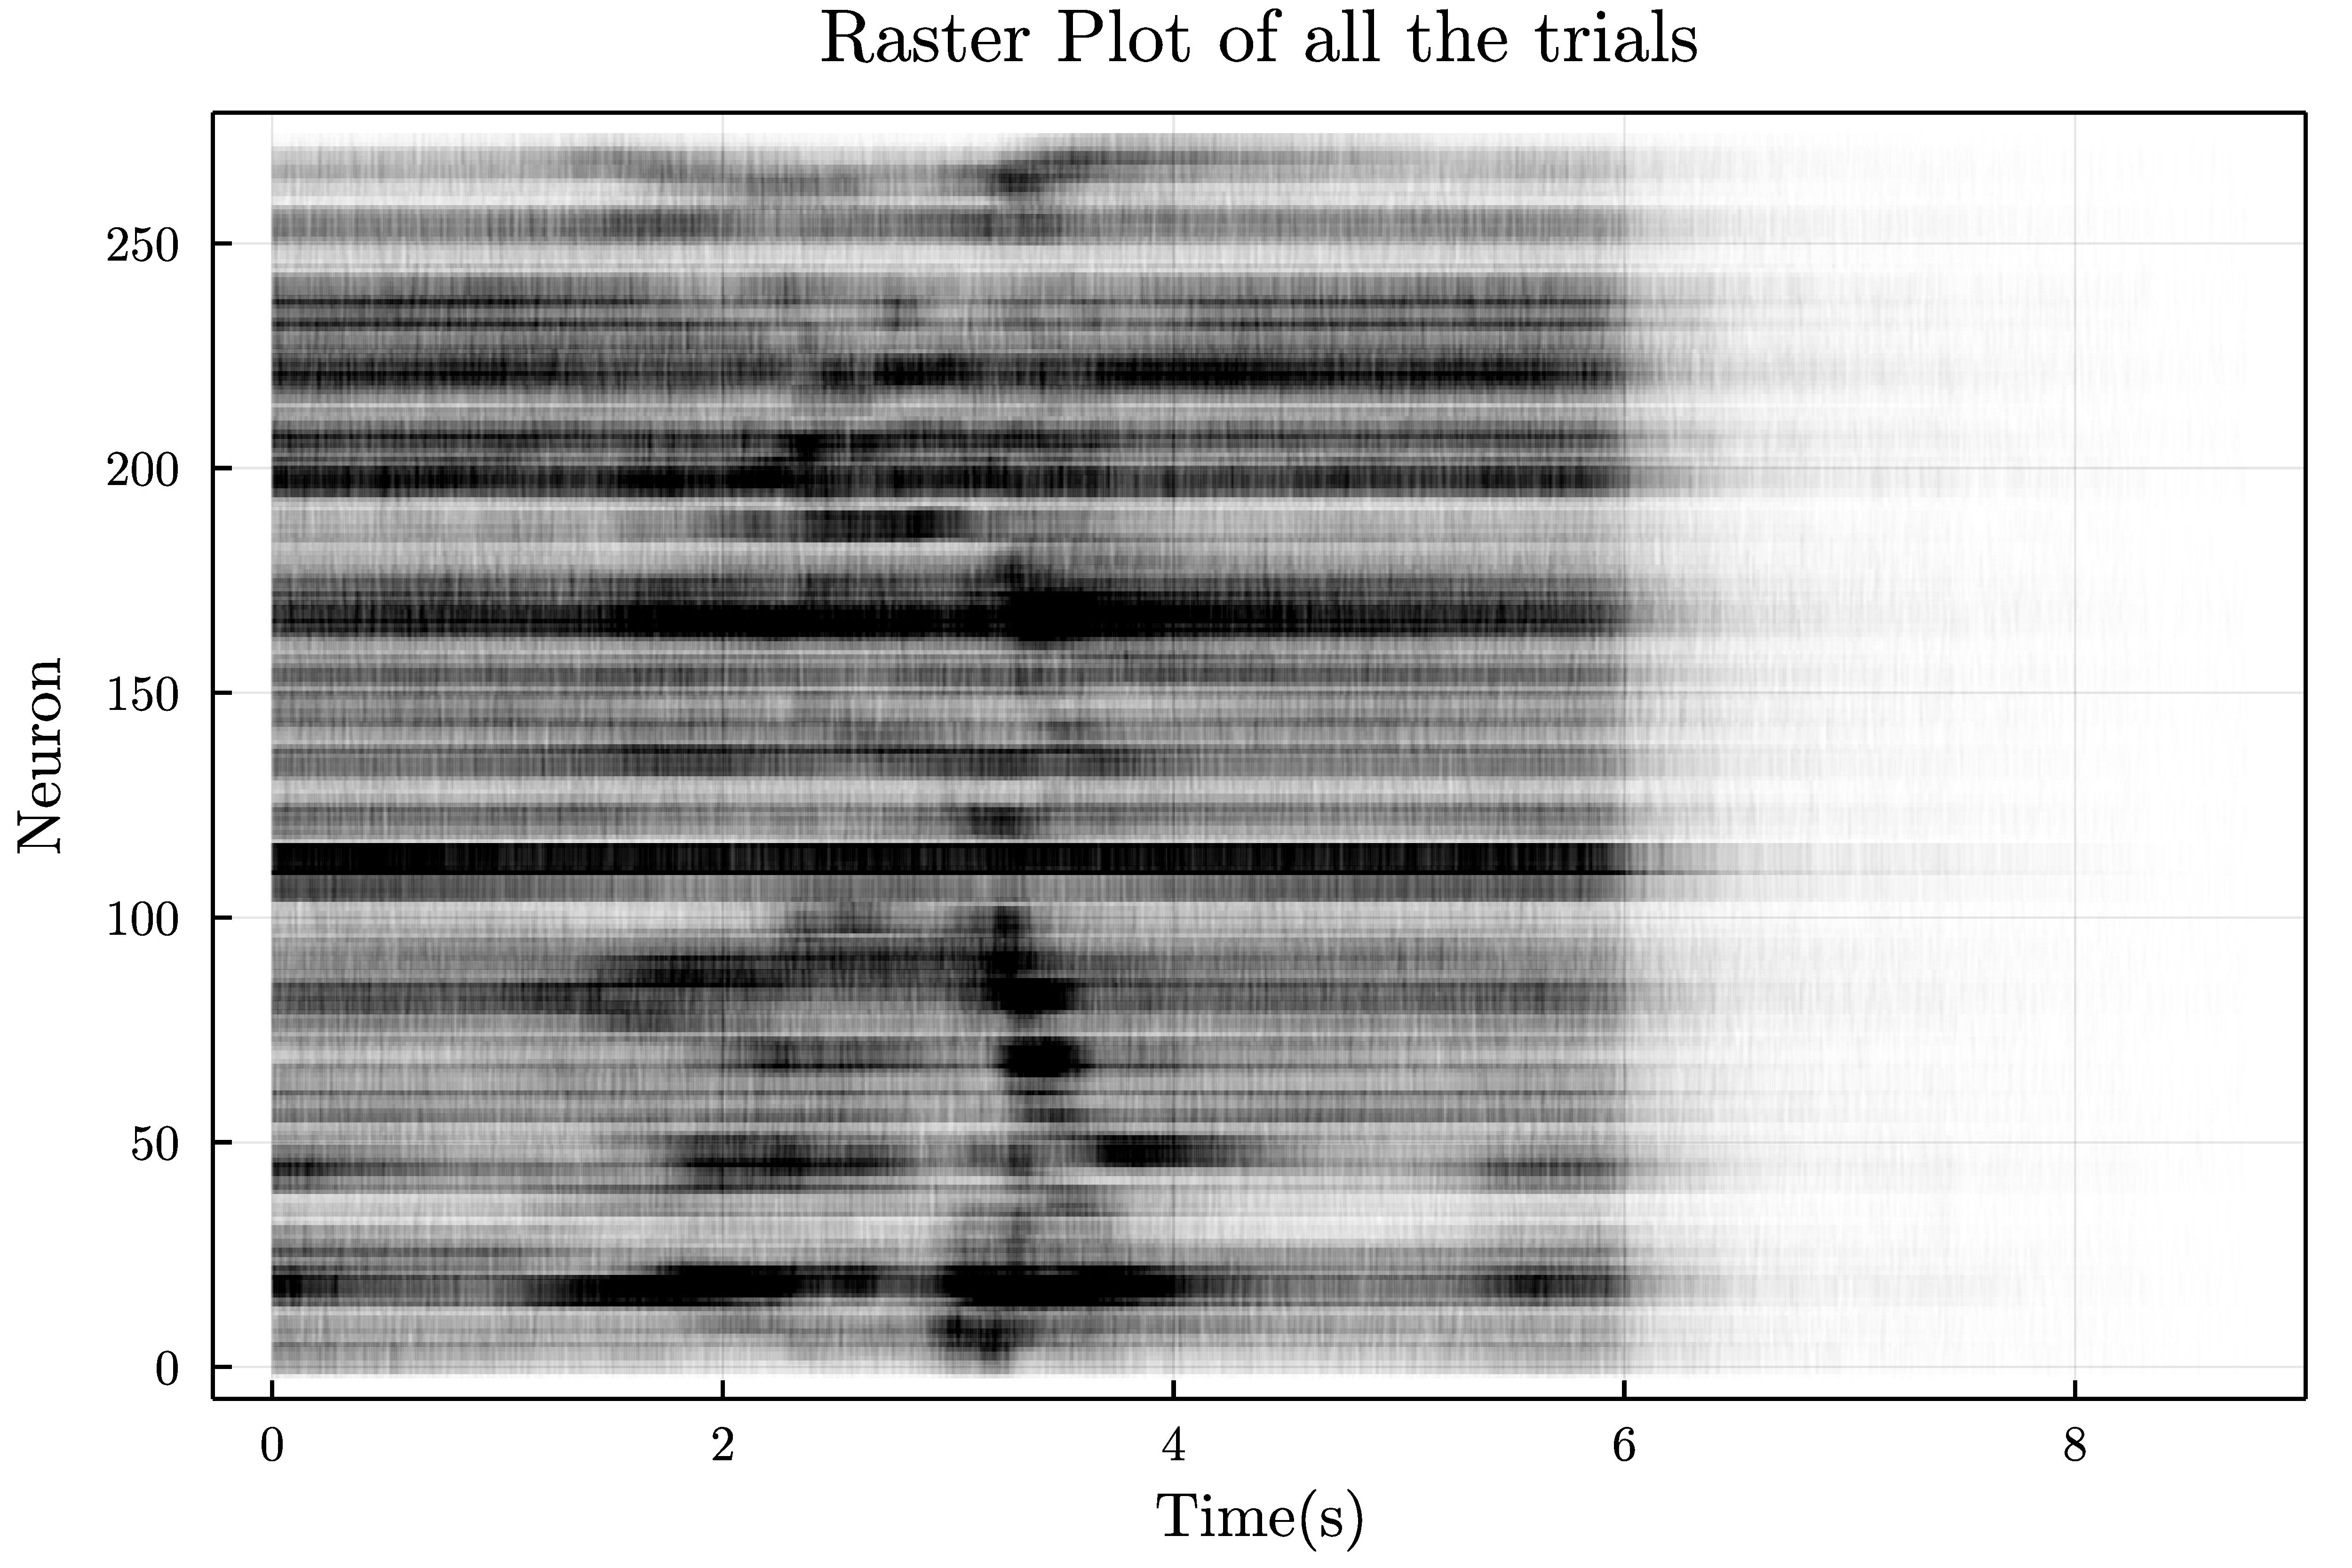
\includegraphics[width=12cm,height=11.4cm]{TotRasterPlot.jpg}
\caption{Raster Plot. The rasters show multiple trials during which a neuron responds to the stimulus.}\label{fig:side}
\end{SCfigure*}
\begin{SCfigure*}[\sidecaptionrelwidth][t]
\centering
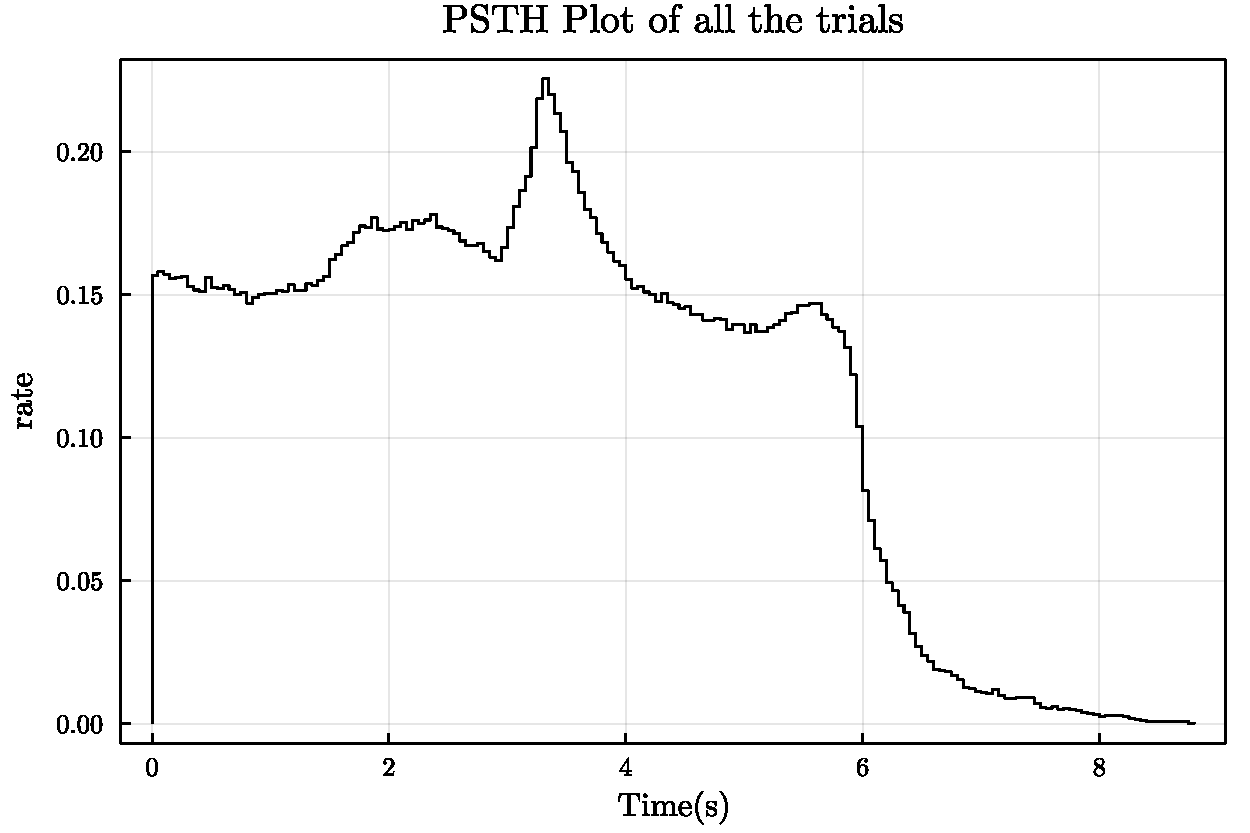
\includegraphics[width=12cm,height=11.4cm]{TotPSTHPlot.pdf}
\caption{PSTH. Firing rates, shown under the raster plot , were constructed from the multiple trials by counting spikes within discrete time bins and averaging over trials.}\label{fig:side}
\end{SCfigure*}

\begin{SCfigure*}[\sidecaptionrelwidth][t]
\centering
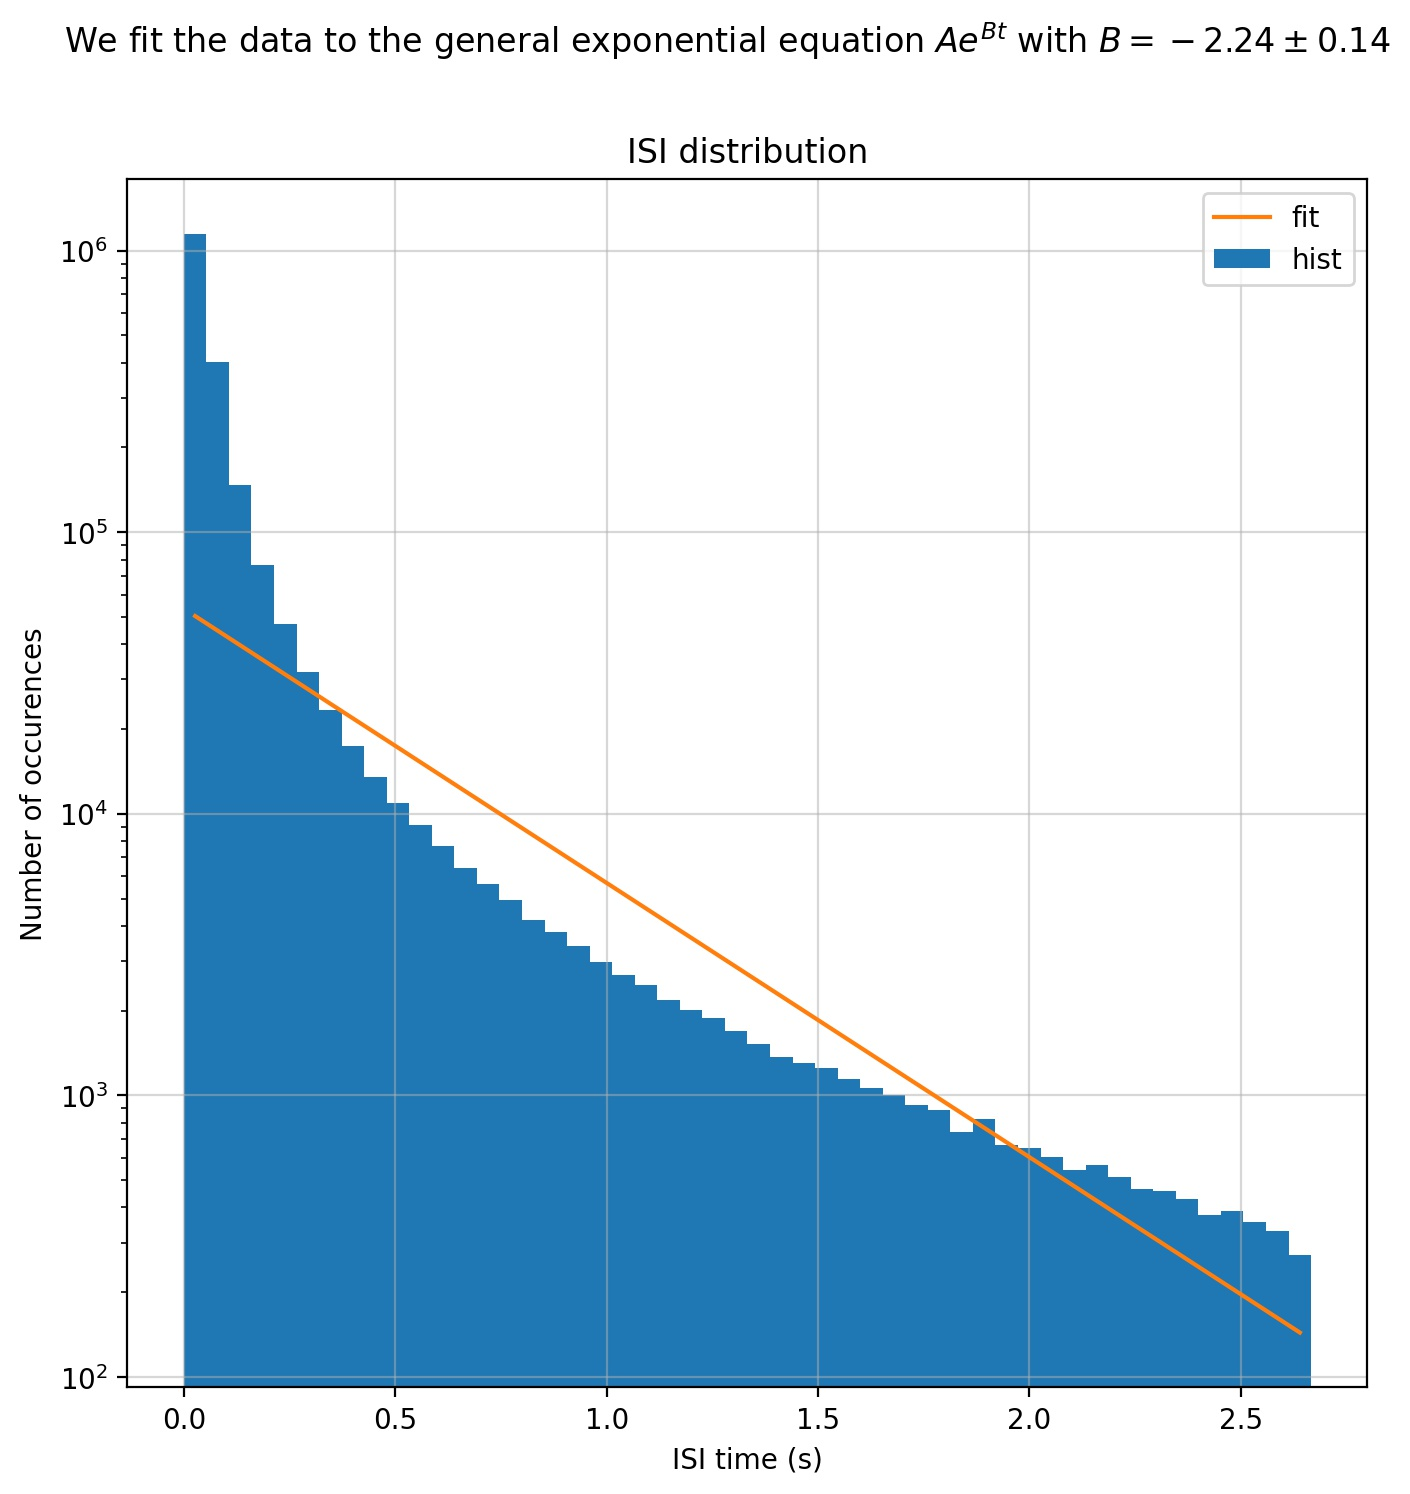
\includegraphics[width=12cm,height=11.4cm]{isi_logfit.jpg}
\caption{The ISI distribution for filtered data. The bin size is between 0 to 8000 indexes. The y- axis then became logarithmic to fit the exponential function.}\label{fig:side}
\end{SCfigure*}

\section*{References}
% Bibliography
\bibliography{references}
\end{document}